\documentclass[t]{beamer}
%\usepackage[orientation=portrait, size=a0, scale=1.0]{beamerposter}
\usepackage[size=custom,width=35,height=40,scale=1]{beamerposter}
%\usepackage[orientation=portrait, size=a4]{beamerposter}
\usepackage{textpos}
\usepackage{tcolorbox}
\usepackage{verbatim} % For using /begin{comment}; /end{comment}
\usepackage{multirow}
\usepackage{booktabs}
\usepackage{graphicx}
\usepackage{lmodern} % Font style
\usepackage{ragged2e} % For using \justify

%\setlength{\paperwidth}{35.0in}
%\setlength{\paperheight}{40.0in}
%\setlength{\textwidth}{34.0in}
%\setlength{\textheight}{39.0in}

\setbeamerfont{frametitle}{size={\fontsize{90}{200}}}
\setbeamerfont{framesubtitle}{size={\fontsize{56}{100}}}
%\setbeamerfont{block title}{size={\fontsize{60}{65}}}
%\setbeamerfont{block body}{size={\fontsize{32}{35}}}
%\setbeamerfont{}
\setbeamerfont{caption}{size={\fontsize{28}{30}}}
\setbeamerfont{tcolorbox title}{size={\fontsize{60}{65}}} % Not working

\setbeamertemplate{frametitle}[default][center]
%\addtobeamertemplate{block begin}{\vspace{-8pt}}{}
%\renewcommand{\figurename}{Fig.}
%\setbeamertemplate{caption}{\raggedright\insertcaption\par}
\setbeamertemplate{caption}[numbered]

\definecolor{frametitlebg}{rgb}{0.0, 0.26, 0.15}
\definecolor{mygray}{rgb}{0.23, 0.27, 0.29}

\setbeamercolor{background canvas}{bg=white}
\setbeamercolor{normal text}{fg=black}
\setbeamercolor{frametitle}{fg=white, bg=frametitlebg}
\setbeamercolor{block title}{fg=white, bg=mygray}
\setbeamercolor{caption name}{fg=mygray}
\setbeamercolor{enumerate item}{fg=mygray}


\begin{document}

%\begin{frame}{%
%    Coronal Seismology: Application to Bright Points in a Coronal Hole}{%
%    Laurel Farris, R. T. James McAteer}
\begin{frame}[t]{}{}
    \begin{tcolorbox}[colback=mygray!5,colframe=mygray!40!mygray,
        title=Coronal Seismology: Application to Bright Points in a Coronal Hole]
        \tcbsubtitle{Laurel Farris, R. T. James McAteer}
    %\vspace{0.5in}
    \begin{columns}
        \column{0.3\textwidth}
        \par\vspace{1in}
        \begin{tcolorbox}[colback=mygray!5,colframe=mygray!40!mygray,
            fonttitle=\sffamily\bfseries\large,
            title=Background \& Motivation]
            The method of coronal seismology is based on the theories of
            ideal magnetohydrodynamics (MHD). Waves and oscillations in the
            solar corona are modelled in a straight cylindar with uniform
            magnetic field. This cylindar acts as a waveguide; examples include
            coronal loops and filaments/prominances.
        \end{tcolorbox}
        \par\vspace{1in}
        \begin{tcolorbox}[colback=mygray!5,colframe=mygray!40!mygray,
            title=Coronal Seismology]
            \begin{enumerate}
                \item Observe disturbances
                \item Measure physical parameters
                \item Identify wave properties
                \item Extract physical parameters
            \end{enumerate}
        \end{tcolorbox}
        \par\vspace{1in}
        \begin{tcolorbox}[colback=mygray!5,colframe=mygray!40!mygray,
            title=Data]
            \begin{figure}
                \vspace{0.1\textwidth}
                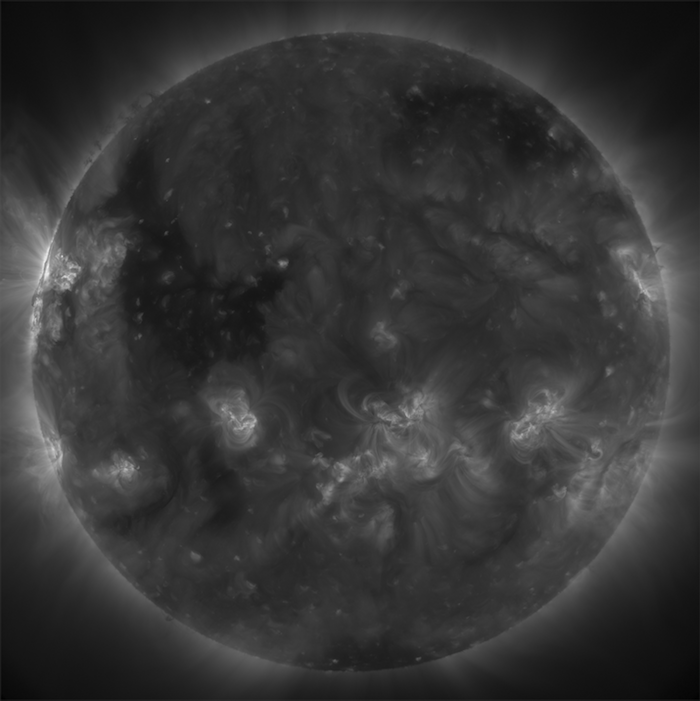
\includegraphics[width=0.8\textwidth]{full_disk.png}
                \caption{Full disk from AIA/\emph{SDO} 193 \AA{}.}
            \end{figure}
            The data analyzed consisted of an hour's worth of images from the
            Atmospheric Imaging Assembly (AIA) on board the \emph{Solar Dynamics
            Observatory (SDO)}.
        \end{tcolorbox}
        \column{0.3\textwidth}
        \par\vspace{1in}
        \begin{tcolorbox}[colback=mygray!5,colframe=mygray!40!mygray,title=Results]
            \begin{figure}
                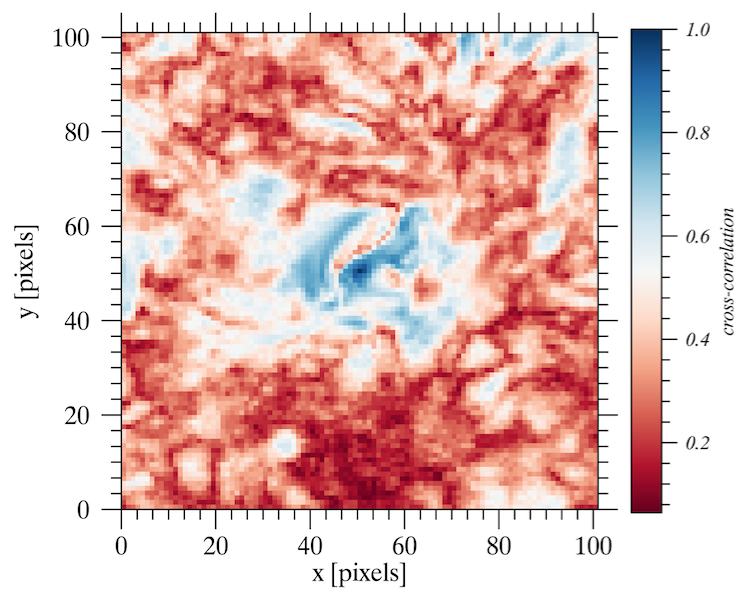
\includegraphics[width=0.9\textwidth]{cc_color_2.png}
                \caption{Cross-correlation image}
            \end{figure}
            \begin{figure}
                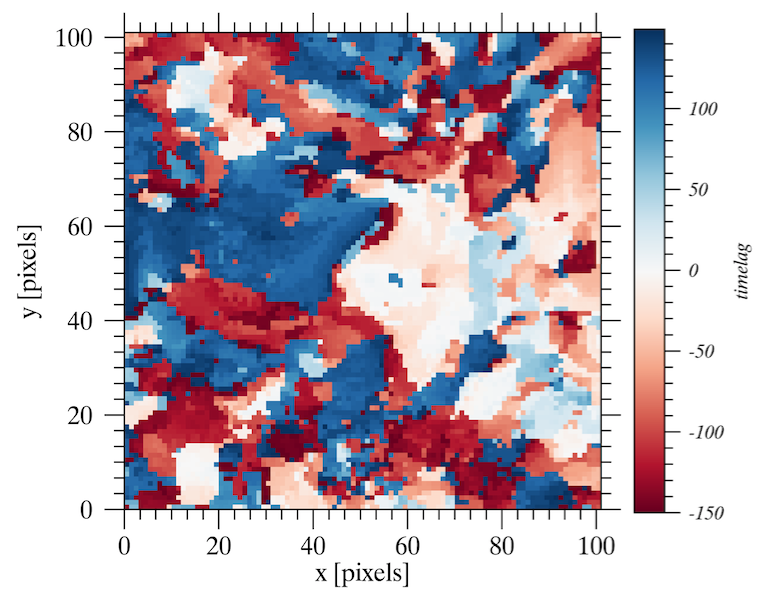
\includegraphics[width=0.9\textwidth]{tt_color_2.png}
                \caption{Timelag image}
            \end{figure}
        \end{tcolorbox}
        \column{0.3\textwidth}
        \par\vspace{1in}
        \begin{tcolorbox}[colback=mygray!5,colframe=mygray!4!mygray,title=Conclusions]
        \end{tcolorbox}
        \par\vspace{1in}
        \begin{tcolorbox}[colback=mygray!5,colframe=mygray!4!mygray,title=Future Work]
        \end{tcolorbox}
        \par\vspace{1in}
        \begin{tcolorbox}[colback=mygray!5,colframe=mygray!4!mygray,title=Acknowledgements]
        \end{tcolorbox}

    \end{columns}
    \vfill
\includegraphics{nmsu.png}
    \end{tcolorbox}
\end{frame}

\end{document}
